%
%
% UCSD Doctoral Dissertation Template
% -----------------------------------
% https://github.com/ucsd-thesis/ucsd-thesis
%
%
% ----------------------------------------------------------------------
% WARNING: 
%
%   This template has not endorced by OGS or any other official entity.
%   The official formatting guide can be obtained from OGS.
%   It can be found on the web here:
%   http://grad.ucsd.edu/_files/academic-affairs/Dissertations_Theses_Formatting_Manual.pdf
%
%   No guaranty is made that this LaTeX class conforms to the official UCSD guidelines.
%   Make sure that you check the final document against the Formatting Manual.
%  
%   That being said, this class has been routinely used for successful 
%   publication of doctoral theses.  
%
%   The ucsd.cls class files are only valid for doctoral dissertations.
%
%
% ----------------------------------------------------------------------
% GETTING STARTED:
%
%   Lots of information can be found on the project wiki:
%   http://code.google.com/p/ucsd-thesis/wiki/GettingStarted
%
%
%   To make a pdf from this template use the command:
%     pdflatex template
%
%
%   To get started please read the comments in this template file 
%   and make changes as appropriate.
%
%   If you successfully submit a thesis with this package please let us
%   know.
%
%
% ----------------------------------------------------------------------
% KNOWN ISSUES:
%
%   Currently only the 12pt size conforms to the UCSD requirements.
%   The 10pt and 11pt options make the footnote fonts too small.
%
%
% ----------------------------------------------------------------------
% HELP/CONTACT:
%
%   If you need help try the ucsd-thesis google group:
%   http://groups.google.com/group/ucsd-thesis
%
%
% ----------------------------------------------------------------------
% BUGS:
%
%   Please report all bugs at:
%   https://github.com/ucsd-thesis/ucsd-thesis/issues
%
%
% ----------------------------------------------------------------------
% More control of the formatting of your thesis can be achieved through
% modifications of the included LaTeX class files:
%
%   * ucsd.cls    -- Class file
%   * uct10.clo   -- Configuration files for font sizes 10pt, 11pt, 12pt
%     uct11.clo                            
%     uct12.clo
%
% ----------------------------------------------------------------------



% Setup the documentclass 
% default options: 12pt, oneside, final
%
% fonts: 10pt, 11pt, 12pt -- are valid for UCSD dissertations.
% sides: oneside, twoside -- note that two-sided theses are not accepted 
%                            by OGS.
% mode: draft, final      -- draft mode switches to single spacing, 
%                            removes hyperlinks, and places a black box
%                            at every overfull hbox (check these before
%                            submission).
% chapterheads            -- Include this if you want your chapters to read:
%                              Chapter 1
%                              Title of Chapter
%
%                            instead of
%                              1 Title of Chapter
\documentclass[12pt,chapterheads]{ucsd}



% Include all packages you need here.  
% Some standard options are suggested below.
%
% See the project wiki for information on how to use 
% these packages. Other useful packages are also listed there.
%
%   http://code.google.com/p/ucsd-thesis/wiki/GettingStarted



%% AMS PACKAGES - Chances are you will want some or all 
%    of these if writing a dissertation that includes equations.
%  \usepackage{amsmath, amscd, amssymb, amsthm}

%% GRAPHICX - This is the standard package for 
%    including graphics for latex/pdflatex.
\usepackage{scrextend}
\usepackage{pslatex}
\usepackage{graphicx}
\usepackage{subfig}

%% CAPTION
% This overrides some of the ugliness in ucsd.cls and
% allows the text to be double-spaced while letting figures,
% tables, and footnotes to be single-spaced--all OGS requirements.
% NOTE: Must appear after graphics and ams math
\makeatletter
\gdef\@ptsize{2}% 12pt documents
\let\@currsize\normalsize
\makeatother
\usepackage{setspace}
\doublespace
\usepackage[font=small, width=0.9\textwidth]{caption}

%% SUBFIG - Use this to place multiple images in a
%    single figure.  Subfig will handle placement and
%    proper captioning (e.g. Figure 1.2(a))
% \usepackage{subfig}

%% TIMES FONT - replacements for Computer Modern
%%   This package will replace the default font with a
%%   Times-Roman font with math support.
% \usepackage[T1]{fontenc}
% \usepackage{mathptmx}

%% INDEX
%   Uncomment the following two lines to create an index: 
% \usepackage{makeidx}
% \makeindex
%   You will need to uncomment the \printindex line near the
%   bibliography to display the index.  Use the command
% \index{keyword} 
%   within the text to create an entry in the index for keyword.
%   To compile a LaTeX document with an index the 'makeindex'
%   command will need to be run.  See the wiki for more details.

%% HYPERLINKS
%   To create a PDF with hyperlinks, you need to include the hyperref package.
%   THIS HAS TO BE THE LAST PACKAGE INCLUDED!
%   Note that the options plainpages=false and pdfpagelabels exist
%   to fix indexing associated with having both (ii) and (2) as pages.
%   Also, all links must be black according to OGS.
%   See: http://www.tex.ac.uk/cgi-bin/texfaq2html?label=hyperdupdest
%   Note: This may not work correctly with all DVI viewers (i.e. Yap breaks).
%   NOTE: hyperref will NOT work in draft mode, as noted above.
% \usepackage[colorlinks=true, pdfstartview=FitV, 
%             linkcolor=black, citecolor=black, 
%             urlcolor=black, plainpages=false,
%             pdfpagelabels]{hyperref}
% \hypersetup{ pdfauthor = {Your Name Here}, 
%              pdftitle = {The Title of The Dissertation}, 
%              pdfkeywords = {Keywords for Searching}, 
%              pdfcreator = {pdfLaTeX with hyperref package}, 
%              pdfproducer = {pdfLaTeX} }
% \urlstyle{same}
% \usepackage{bookmark}


%% CITATIONS
% Sets citation format
% and fixes up citations madness
\usepackage{microtype}  % avoids citations that hang into the margin


%% FOOTNOTE-MAGIC
% Enables footnotes in tables, re-referencing the same footnote multiple times.
\usepackage{footnote}
\makesavenoteenv{tabular}
\makesavenoteenv{table}


%% TABLE FORMATTING MADNESS
% Enable all sorts of fun table tricks
\usepackage{rotating}  % Enables the sideways environment (NCPW)
\usepackage{array}  % Enables "m" tabular environment http://ctan.org/pkg/array
\usepackage{booktabs}  % Enables \toprule  http://ctan.org/pkg/array


\usepackage{url}
\begin{document}

%% FRONT MATTER
%
%  All of the front matter.
%  This includes the title, degree, dedication, vita, abstract, etc..
%  Modify the file template_frontmatter.tex to change these pages.
%
%
% UCSD Doctoral Dissertation Template
% -----------------------------------
% http://ucsd-thesis.googlecode.com
%
%


%% REQUIRED FIELDS -- Replace with the values appropriate to you

% No symbols, formulas, superscripts, or Greek letters are allowed
% in your title.
\title{Separation of a Known Speaker's Voice with a Convolutional Neural Network}

\author{Michael Threet}
\degreeyear{\the\year}

% Master's Degree theses will NOT be formatted properly with this file.
\degreetitle{Master of Science}

\field{Electrical and Computer Engineering}
\specialization{Signal and Image Processing}  % If you have a specialization, add it here

\chair{Professor Truong Nguyen}
% Uncomment the next line iff you have a Co-Chair
% \cochair{Professor Cochair Semimaster}
%
% Or, uncomment the next line iff you have two equal Co-Chairs.
%\cochairs{Professor Chair Masterish}{Professor Chair Masterish}

%  The rest of the committee members  must be alphabetized by last name.
\othermembers{
Professor William Hodgkiss\\
Professor Bhaskar Rao
}
\numberofmembers{3} % |chair| + |cochair| + |othermembers|


%% START THE FRONTMATTER
%
\begin{frontmatter}

%% TITLE PAGES
%
%  This command generates the title, copyright, and signature pages.
%
\makefrontmatter

%% DEDICATION
%
%  You have three choices here:
%    1. Use the ``dedication'' environment.
%       Put in the text you want, and everything will be formated for
%       you. You'll get a perfectly respectable dedication page.
%
%
%    2. Use the ``mydedication'' environment.  If you don't like the
%       formatting of option 1, use this environment and format things
%       however you wish.
%
%    3. If you don't want a dedication, it's not required.
%
%
% \begin{dedication}
%   To two, the loneliest number since the number one.
% \end{dedication}


% \begin{mydedication} % You are responsible for formatting here.
%   \vspace{1in}
%   \begin{flushleft}
% 	To me.
%   \end{flushleft}
%
%   \vspace{2in}
%   \begin{center}
% 	And you.
%   \end{center}
%
%   \vspace{2in}
%   \begin{flushright}
% 	Which equals us.
%   \end{flushright}
% \end{mydedication}



%% EPIGRAPH
%
%  The same choices that applied to the dedication apply here.
%
%\begin{epigraph} % The style file will position the text for you.
%  \emph{A careful quotation\\
%  conveys brilliance.}\\
%  ---Smarty Pants
%\end{epigraph}

% \begin{myepigraph} % You position the text yourself.
%   \vfil
%   \begin{center}
%     {\bf Think! It ain't illegal yet.}
%
% 	\emph{---George Clinton}
%   \end{center}
% \end{myepigraph}


%% SETUP THE TABLE OF CONTENTS
%
\tableofcontents
\listoffigures  % Comment if you don't have any figures
\listoftables   % Comment if you don't have any tables



%% ACKNOWLEDGEMENTS
%
%  While technically optional, you probably have someone to thank.
%  Also, a paragraph acknowledging all coauthors and publishers (if
%  you have any) is required in the acknowledgements page and as the
%  last paragraph of text at the end of each respective chapter. See
%  the OGS Formatting Manual for more information.
%
%\begin{acknowledgements}
% Thanks to whoever deserves credit for Blacks Beach, Porters Pub, and
% every coffee shop in San Diego.
%
% Thanks also to hottubs.
%\end{acknowledgements}


%% VITA
%
%  A brief vita is required in a doctoral thesis. See the OGS
%  Formatting Manual for more information.
%
%\begin{vitapage}
%\begin{vita}
%  \item[2002] B.~S. in Mathematics \emph{cum laude}, University of Southern North Dakota, Hoople
%  \item[2002-2007] Graduate Teaching Assistant, University of California, San Diego
%  \item[2007] Ph.~D. in Mathematics, University of California, San Diego
%\end{vita}
%\begin{publications}
%  \item Your Name, ``A Simple Proof Of The Riemann Hypothesis'', \emph{Annals of Math}, 314, 2007.
%  \item Your Name, Euclid, ``There Are Lots Of Prime Numbers'', \emph{Journal of Primes}, 1, 300 B.C.
%\end{publications}
%\end{vitapage}


%% ABSTRACT
%
%  Doctoral dissertation abstracts should not exceed 350 words.
%   The abstract may continue to a second page if necessary.
%
\begin{abstract}
	Source Separation (SS) refers to a problem in signal processing where two or more mixed signal sources must be separated into their individual components. While SS is a challenging problem, it may be simplified by making assumptions on the signals that are present and the methods used to mix the signals. One example of this is to limit the range of signals to human voices and to limit the total number of speakers (through either estimation or always having a set number of speakers). This paper assumes that the speech from two speakers is mixed at one microphone, with the voice of one speaker (Speaker 1) being present in all recordings. Traditional approaches to the SS problem typically involve array processing and time-frequency methods to perform the separation. Once such example is Non-Negative Matrix Factorization (NMF), which attempts to factor a spectrogram into frequency basis vectors and time weights for each speaker. This paper will explore the use of a Convolutional Neural Network (CNN) to learn effective separation of Speaker 1's voice from a variety of other speakers and background noises. The CNN will prove to be much more effective than NMF due to the ability of the CNN to learn a representative feature space of Speaker 1's speech.
\end{abstract}


\end{frontmatter}






%% DISSERTATION

% A common strategy here is to include files for each of the chapters. I.e.,
% Place the chapters is separate files: 
%   chapter1.tex, chapter2.tex
% Then use the commands:
%   \include{chapter1}
%   \include{chapter2}
%
% Of course, if you prefer, you can just start with
%   \chapter{My First Chapter Name}
% and start typing away. 


\section{Introduction}
\label{sec:intro}
General Source Separation (SS) is difficult, but with assumptions made on the signals that are present and their mixing methods, it becomes a much more tractable problem. In this paper, assumptions were made that all signals were a mixture of two human voices at a single microphone, and that the voice of  a certain speaker (Speaker 1) was present in every signal. The proposed solution is a Convolutional Neural Network (CNN) that is trained to separate Speaker 1's voice from the raw audio mixture recorded at the microphone. By keeping Speaker 1's voice constant through all training steps, the CNN will learn the underlying features of Speaker 1's voice and will be able to separate Speaker 1's voice from a variety of other voices. While many SS algorithms use time-frequency processing to acquire a better relationship of the mixed signals, this CNN method is more unique in its ability to take raw audio as an input and return the separated raw audio as an output. Non-Negative Matrix Factorization (NMF) for example, factors the spectrogram of the mixed signals into matrices whose columns and rows correspond to the time-frequency and activity components of each signal present.


\section{Background}
\subsection{The Dataset and Evaluation}
The dataset used in this paper was borrowed from the Language and Speech Lab's 1\textsuperscript{st} Speech Separation Challenge \cite{laslab}. The dataset consists of a 34 individual speakers uttering short sentences, along with combinations of these speakers' voices in a variety of patterns. This paper focused solely on separating Speaker 1's voice from a number of different  speakers. The dataset provided both a mixed version and a clean version of Speaker 1's voice for each example, which allowed for the quality of reconstruction to be measured. 

The dataset provided the mixtures at varying Signal-to-Noise Ratios (SNRs), and this paper used the whole range. All reconstructions of Speaker 1's voice were evaluated on the Root Mean Squared Error (RMSE) between the separated voice and the original voice.

\subsection{Non-Negative Matrix Factorization}
Non-negative Matrix Factorization attempts to factor an $n \times m$ matrix $A$ with all $A_{ij} \geq 0$ into two matrices: $W$, an $n \times k$ matrix and $H$, a $k \times m$ matrix. For speech separation, $A$ is the magnitude of the spectrogram of the mixed signals and $k$ is the estimated number of speakers. For this paper, the assumption was made that $k=2$ in all cases. Since $A$ is a magnitude spectrogram, it satisfies the condition that $A_{ij} \geq 0$. For a given spectrogram magnitude $A$, $n$ is the number of Discrete Fourier Transform (DFT) frequency bins, and $k$ is the number of discrete time steps that the DFT was taken at.

The objective of NMF is to minimize the Frobenius Norm between the original matrix $A$ and the reconstructed matrix $WH$ (i.e. $\| A - WH\|_2$). The Frobenius norm is defined as:

\begin{equation}
\| Q \|_2 = \sqrt{\sum\limits_{i} \sum\limits_{j} Q_{ij}^2}
\end{equation}

Given the objective function, it is possible to solve for $W$ and $H$ iteratively with the following multiplicative update equations and random initializations for $W$ and $H$ \cite{Lee00algorithmsfor}:

\begin{equation}
W \leftarrow W \circ \frac{AH'}{WHH'}
\end{equation}
\begin{equation}
H \leftarrow H \circ \frac{W'A}{W'WH'}
\end{equation}

where $A \circ B$ and $\frac{A}{B}$ represent elementwise multiplication and division respectively. With enough iterations, the Frobenius objective should converge to within a small threshold.

NMF is useful due to its simple iterative implementation and because spectrogram magnitude matrices by definition satisfy the non-negative condition.  Additionally, the matrices $W$ and $H$ have useful signal interpretations. The columns of $W$ form $k$ frequency basis vectors for the spectrogram $A$, while the rows of $H$ act as time-varying activations for the frequency bases in $W$. The spectrograms of the $k$ independent signals are then estimated as:

\begin{equation}
X_i = W_{:i}H_{i:}, i=1,...,k
\end{equation}

where $W_{:i} $represents the the $i^{th}$ column of $W$, and $H_{i:} $represents the the $i^{th}$ row of $H$. In essence, each source is approximated as a basis spectrogram $X_i$ for the total spectrogram $A$. The original time-series speech signals are then recovered by multiplying each of the individual magnitude spectrograms $X_i$ with the phase of the spectrogram corresponding to $A$, and finding the inverse of the complex-valued spectrogram.

\subsection{Convolutional Neural Networks}
Convolutional Neural Networks generally use a combination of convolution, activation, and pooling layers to estimate a desired output signal given an input signal. CNNs will essentially learn a mapping from an input signal to an output signal, which for this paper were the mixed signal containing Speaker 1's voice and another voice and Speaker 1's voice, respectively. The benefit of a CNN is that the weights of all the convolutional filters do not need to be hand-designed. Instead, they are learned iteratively during a training process. Figure \ref{fig:cnn_model} shows the CNN used in this paper.

\begin{figure}[h] 
  \centering
  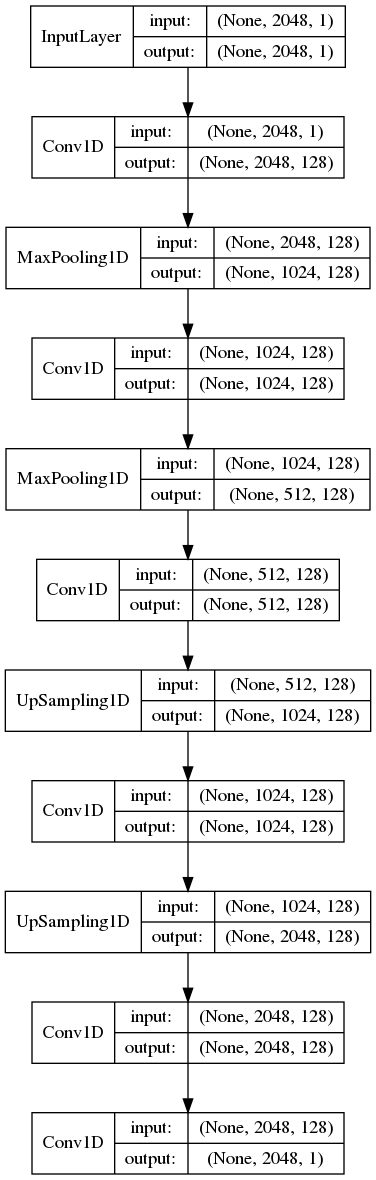
\includegraphics[width=0.25\textwidth]{pics/model}
  \caption[The CNN model and its layers]
{The CNN model with its layers. The graph shows the input and output size of each layer, along with the layer name/type.}
  \label{fig:cnn_model}
\end{figure}

A convolutional layer consists of a collection of filter kernels, each with their own adjustable/learnable weights. For example, the first convolutional layer in Figure \ref{fig:cnn_model}, contains 128 filter kernels, each of which is convolved with the input signal of length 2048. This in turn gives the first convolutional layer 128 outputs, each of length 2048.

Although not listed in Figure \ref{fig:cnn_model}, each convolutional layer is followed by an activation layer. These activations apply non-linear functions to the convolutional layer outputs, which allow for greater feature learning by the network. If no non-linearities were applied, the CNN could be viewed as a linear system, which would decrease the effectiveness of adding additional layers. For this paper, hyperbolic tangent non-linearities were used after each convolutional layer, except for the last layer, which had a linear activation applied (so that the output signal can take on a more linear range of values).

The pooling layers downsample the signals passing through the CNN. The model in Figure \ref{fig:cnn_model} has max-pooling layers and a downsampling rate of 2, which translates to only the maximum value between pairs of consecutive samples remaining. Ideally, the convolutional layers will amplify the samples related to Speaker 1's voice, and max-pooling will retain only those samples.

The upsampling layers serve to undo the effects of the downsampling layers, so that the output signal has the same length as the input signal. The upsampling layers learn upsampling filters that best reconstruct Speaker 1's voice given the previous layers' outputs.

The loss used in the CNN was a combination of the RMSE between the CNN output and Speaker 1's true speech signal, and the RMSE between the DFTs of the CNN output and Speaker 1's true speech signal. This allowed for both the time and frequency components of the reconstructed speech signal to be evaluated, while still making the network loss easy to compute.

The true power of a CNN is that, given an output error, the best updates to the filter weights in the network can be computed through backpropagation. Each layer in the CNN will is used to compute the output of the network, so the partial derivatives of each layer with respect to each other and the output can be computed. In this sense, the error at the output can be propagated backwards through the CNN to update the filter weights at each layer.


\section{Technical Approach and Results}
All experimentation in this paper was done with Python 3.6. Python's librosa library was used for all audio processing, as it provides nice tools for loading, manipulating, and saving audio files.

\subsection{NMF}
The NMF algorithm used in this paper was always used with no initializations for $W$ and $H$, a Frobenius norm objective, a maximum of 200 iterations, and with the number of components always set to two. The input audio signal was comprised of 32000 samples, and the spectrogram was computed using a segment size of 512, a DFT length of 512, an overlap of 128, and Kaiser window with $\beta = 14$.

The magnitude and phase of the resulting spectrogram were taken, and NMF was applied to the spectrogram magnitude with the parameters mentioned above. The resulting separated spectrogram magnitudes were then computed using the output of NMF, and the separated audio signals were obtained by taking the inverse spectrograms of the spectrogram magnitudes multiplied by the original spectrogram's phase.

The RMSE between the estimate of Speaker 1's separated speech and Speaker 1's actual speech was then taken and recorded as the metric for reconstruction.

\subsection{CNN}
The architecture of the CNN in this paper is shown in Figure \ref{fig:cnn_model}. The filters in all convolutional layers had a kernel size of 16 and hyperbolic tangent activations applied, except for the final convolutional layer, which had a no activation (i.e. a linear activation) applied. Unlike the NMF processing, the input to the CNN was cut into segments of length 128, with no windowing applied. The CNN was trained on 2,000 example files, each with 32,000 samples. After training, the CNN was evaluated on 500 separate example files, each with 32,000 samples. The evaluation files were chosen randomly from the whole dataset so that a representative portion was obtained.


\subsection{Results}
Table \ref{table:results} shows a summary of the results  for NMF and the CNN. Note that all signals were normalized so that maximum value was one before the RMSE was taken.

\vspace{0.25in}
\begin{table}[!ht]
\caption{Summary of reconstruction results (given in RMSE) at a variety of SNRs}

\vspace{-0.25in}
\begin{center}
\begin{tabular}{| c | c | c |  c | c | c |}

\hline
Method & -6 dB & -3 dB & 0 dB & 3 dB & 6dB \\

\hline
NMF & 0.15 & 0.12 & 0.10 & 0.08 & 0.04 \\

\hline
CNN & 0.13 & 0.09 & 0.06 & 0.03 & 0.01 \\

\hline
\end{tabular}
\end{center}
\label{table:results}
\end{table}


\section{Conclusion}
As seen in Table \ref{table:results}, the CNN performs better at all SNRs. Both the NMF algorithm and the CNN perform better as the SNR increases, which makes sense due to both methods having to do less work to transform the input mixed signal into the separated signal. While Table \ref{table:results} shows that the two methods are not too far off in their reconstruction errors, the graphical results reveal a different result.

Figure \ref{fig:sim_res} shows a reconstruction example where both NMF and the CNN perform decently well at reconstruction. While neither method is perfect, and both methods tend to look more like the mixed signal in areas of uncertainty, the output is generally smooth and natural.

\begin{figure}[h]
    \begin{minipage}{.5\linewidth}
        \centering
        \subfloat[]{\label{main:a}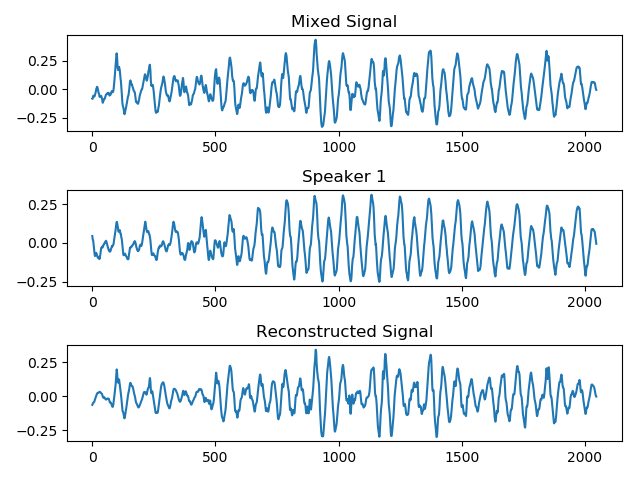
\includegraphics[scale=.45]{pics/nnmf1}}
    \end{minipage}%
    \begin{minipage}{.5\linewidth}
        \centering
        \subfloat[]{\label{main:b}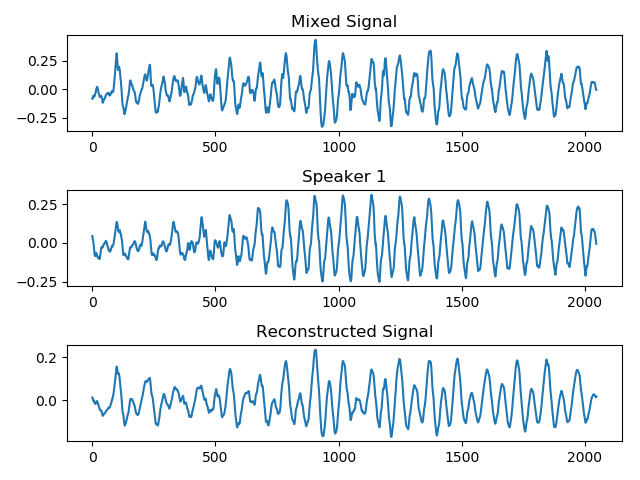
\includegraphics[scale=.45]{pics/cnn1}}
    \end{minipage}
    \caption{ a) The results using NMF b) The results using the CNN}
    \label{fig:sim_res}
\end{figure}

A more typical reconstruction example is shown in Figure \ref{fig:diff_res}. In most cases, NMF was not able to effectively reconstruct Speaker 1's voice in a realistic manner, even when the mixed signal was comprised mainly of only Speaker 1's voice. The CNN, on the other hand, was actually able to perform a small amount of denoising at the end of mixed signal.

\begin{figure}[h]
    \begin{minipage}{.5\linewidth}
        \centering
        \subfloat[]{\label{main:a}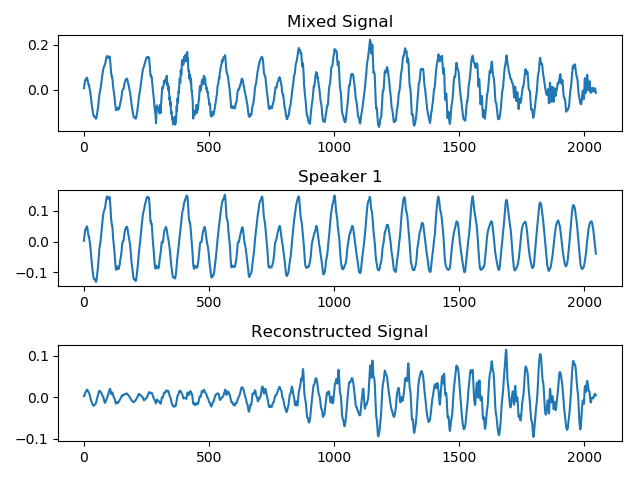
\includegraphics[scale=.45]{pics/nnmf2}}
    \end{minipage}%
    \begin{minipage}{.5\linewidth}
        \centering
        \subfloat[]{\label{main:b}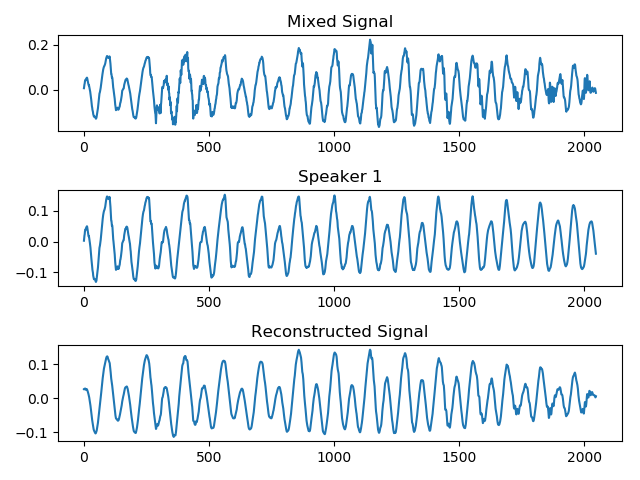
\includegraphics[scale=.45]{pics/cnn2}}
    \end{minipage}
    \caption{ a) The results using NMF b) The results using the CNN}
    \label{fig:diff_res}
\end{figure}

In general, the CNN produced much smoother and more realistic results. The CNN has three advantages over NMF: it can use nonlinear methods, it can use a variety of loss functions, and it can use a large amount of training examples to learn more robust reconstructions.

The CNN applies nonlinear activations after each convolutional layer, which allows for nonlinear approximations to be made. Conversely, NMF relies on a linear matrix factorization, which places limitations on the reconstruction quality of Speaker 1's voice.

The CNN loss function for this experiment was a combination of the difference in the reconstruction and Speaker 1's original speech in both the time and frequency domains. This allows for better phase reconstruction in the reconstructed signal. NMF, meanwhile, is only able to use the spectrograms of the original and reconstructed speech signals, which ignores any phase information, and does not consider time-domain accuracy.

Finally, the CNN is able to use the thousands of past examples it has seen to influence the reconstruction of future signals. The CNN can learn 
common patterns or features in Speaker 1's voice and reconstruct them more easily as training time increases. NMF, on the other hand, does not keep track of any past examples, so only the current input is weighted for consideration. In other words, NMF cannot learn any patterns or features of Speaker 1's voice.






%% APPENDIX
\appendix



%% END MATTER
% \printindex %% Uncomment to display the index
% \nocite{}  %% Put any references that you want to include in the bib 
%               but haven't cited in the braces.
\bibliographystyle{alpha}  %% This is just my personal favorite style. 
%                              There are many others.
%\setlength{\bibleftmargin}{0.25in}  % indent each item
%\setlength{\bibindent}{-\bibleftmargin}  % unindent the first line
%\def\baselinestretch{1.0}  % force single spacing
%\setlength{\bibitemsep}{0.16in}  % add extra space between items
\bibliography{template}  %% This looks for the bibliography in template.bib 
%                          which should be formatted as a bibtex file.
%                          and needs to be separately compiled into a bbl file.
\end{document}

